\documentclass[times, utf8, diplomski]{fer}
\usepackage{booktabs}
\graphicspath{{./img/}}

\begin{document}

% TODO: Navedite broj rada.
\thesisnumber{2451}

% TODO: Navedite naslov rada.
\title{Klasifikacija pokreta ljudskog tijela temeljena na podacima s inercijskih senzora}

% TODO: Navedite vaše ime i prezime.
\author{Ivan Trubić}

\maketitle

% Ispis stranice s napomenom o umetanju izvornika rada. Uklonite naredbu \izvornik ako želite izbaciti tu stranicu.
\izvornik

% Dodavanje zahvale ili prazne stranice. Ako ne želite dodati zahvalu, naredbu ostavite radi prazne stranice.
\zahvala{}

\tableofcontents

\chapter{Uvod}
Karakteristike pokreta ljudskoga tijela vrlo su individualne te ovise o mnogo čimbenika kao što su genetika, odgoj te
fizička sprema. Ti pokreti su toliko jedinstveni da se mogu koristiti za identifikaciju osoba dok su s druge strane
toliko slični da čak i manje devijacije u tim pokretima također mogu ukazivati na neke zdravstvene probleme.
Ljudski pokreti mogu se klasificirati na razne načine koristeći računalni vid ili razne senzore postavljene na
ljudskome tijelu. Svaka od metoda ima svoju granu primjene kao: identifikacija osoba temeljenog na hodu koristeći
računalni vid na nadzornim kamerama \citep{surveillance}, pračenje pokreta igrača u interakciji sa igrama u virtualnoj stvarnosti \citep{VR},
korištenje inercijskih (IMU) senzora za precizno snimanje hoda u svhu otkrivanja bolesti i rehabilitacije te mnoge druge.

Klasifikacija pokreta vrlo je složen problem te kao takav nema dobro rješenje koristeći klasične algoritme. Razvojem moči računala
te metoda strojnoga učenja ovaj problem postaje rješiv. Za snimanje pokreta može se koristiti kamera ili senzori.
Koristeći kameru, na snimci se koriste metode računalnog vida te se traže karakteristike ljudskog tijela kako bi se na snimci
prepoznala osoba te koristeći te karakteristične točke analizira se hod. Također, kamera može snimati osobu sa posebno postavljenim
vizualnim oznakama po djelovima tijela te koristeći te vizualne oznake analizirati pokrete. Nedostatak kamera je taj što snimaju iz
jedne perspektive te zbog toga može doći do okluzije oznaka. Inercijski (IMU) senzori eliminiraju kamere te ne pate od problema okluzije.
Inercijski senzori su relativno jeftini i mali uređaji koji se postave na ključne djelove ljudskoga tijela te pružaju vrlo dobar uvid
u ljudske pokrete. Primjerice mogu se staviti na ruke te upravljati igrama i uređajima ali se mogu koristiti i u medicinske svrhe za
analizu hoda i diagnosticiranje zdravstvenih problema kao i za provođenje terapijskih vježbi bez nadzora stručnjaka.
Ovaj rad će se više fokusirati na medicinski aspekt klasifikacije pokreta, preciznije analizu hoda (\textit{eng.} gait) i terapiju koljena.



\chapter{Razrada}

\section{Bolesti koljena}

\section{Dosadašnja rješenja}

\section{Rješenje koristeći IMU senzore}

\section{Analiza IMU senzora}

\section{Analiza dostupnih baza podataka}

\section{Stvaranje vlastite baze podataka}
Za stvaranje vlastite baze podataka potrebno je definirati svrhu i ciljeve te baze a zatim odrediti metodu prikupljanja podataka. U ovome će radu
fokus biti primarno na stvaranje baze podataka korisne za analizu pokreta koja bi se mogla upotrijebiti u svrhe fizikalne terapije koljena.
Za snimanje općenitih pokreta može se iskoristiti mnogo senzora postavljenih po cijelome tijelu ali za potrebe snimanja jednoga zgloba potrebno je 
koristiti dva senzora, po jedan sa svake strane uda kojeg zglob povezuje. U konkretnom primjeru koljena to su nadkoljenica i potkoljenica.

Ovisno o razini preciznosti, cjeni i dostupnosti potrebno je odabrati i same senzore za prikupljanje podataka. Redovito se sustavi senzora
za istraživačke svrhe rade baš za tu namjenu te postoji mnogo sustava otvorenog koda i otvorenih komponenti koji se mogu iskoristiti. Razni
proizvođači nude i svoja već gotova komercijalna rješenja za koje garantiraju rad i pružaju podršku ali takvi sustavi ponekad nisu adekvatni za
istraživačke svrhe zbog svoje zatvorenosti i potencijalnog manjka interoperabilnosti sa drugim uređajima i programima. U ovome radu, zbog jednostavnosti,
koristiti će se pametni telefon.

Tipičan životni vijek jednog pametnog telefona u prosjeku je dvije godine nakon čega korisnici redovito kupuju nove modele jer stariji postaju neadekvatni
po pitanju trajanja baterije, količine memorije, performansama komponenti i slično. Svaki takav stariji model telefona vrlo često stoji nekorišten iako je još uvijek
funkcionalan. Gotovo svaki pametni telefon u sebi sadrži IMU senzor te u sebi već ima povezivosti poput \textit{WiFi i Bluetooth}. Uzimajući u obzir
također da pametni telefoni imaju i ugrađenu bateriju koja može još uvijek biti dovoljno dugotrajna, ekran osjetljiv na dodir kao metodu interakcije i to 
sve ukomponirano u uređaj koji svojim dimenzijama stane u džep dolazimo do zaključka da su pametni telefoni i više nego adekvatni za prikupljanje podataka.
Također, vrlo je realna pretpostavka da svaka osoba ima pristup minimalno jednome, vjerojatno i dva pametna telefona što čini prikupljanje velike količine
podataka od većeg broja sudionika znatno jednostavnijim. Koristeći držaće pametnog telefona za trčanje ili marama, uređaji se mogu postaviti osobi na bilo koji
dio tijela vrlo jednostavno i svaka bi osoba iz svoga doma mogla pridonjeti stvaranju baze podataka.

Aplikacija koja očitava vrijednosti može biti napravljena posebno, no na tržištu postoje gotove aplikacije, redovito otvorenoga koda, koje se već time bave.
Bitno je pronaći odgovarajuću aplikaciju no u slučaju da takva ne postoji potrebno je izraditi svoju. Mnoge aplikacije u trgovini ne nude selekciju samo određenih senzora
već snimaju sve senzore kojima pametni telefon raspolaže, te u većini slučajeva nude formatiranu pohranu podataka isključivo u memoriju uređaja što je vrlo neadekvatno ako bi se uređaji
koristili primjerice za obradu informacija u stvarnome vremenu ili za centralizirano prikupljanje podataka primjerice na računalo. Neke od takvih aplikacija su
\textit{Sensor Data} i \textit{phyphox} koje se koriste u edukaciji te su u doba COVID pandemije nezamjenjivi alati za vršenje fizikalnih eksperimenata kao dio
školske zadaće. Nedostatak ovih aplikacija je taj što sve podatke snimaju na lokalnoj memoriji uređaja te nisu primjerene za obradu podataka u stvarnome vremenu.
Aplikacija \textit{Sensorstream IMU+GPS} ne nudi grafičke prikaze podataka već u svojoj vrlo bazičnoj funkcionalnosti nudi odabir senzora uz prikaz trenutnih
vrijednosti istih te odabir akcije koju želimo napraviti sa tim podacima. Ponuđene su funkcije spremanja vrijednosti u CSV (\textit{Comma separated value}) formatu,
slanje podataka koristeći UDP protokol te kombinaciju oboje. Za slanje podataka korištenjem UDP protokola potrebno je navesti određenu IP adresu uređaja te \textit{port} na
kojemu uređaj očekuje promet. Također nudi 4 frekvencije uzorkovanja označene sa \textit{slow, medium, fast i fastest}. Te frekvencije uzorkovanja nisu dobro dokumentirane
te nigdje nije navedeno koliko one iznose zapravo. Za mjerenje tih frekvencija može se iskoristiti alat \textit{wireshark}. Wireshark je alat otvorenoga koda koji
služi za analizu mrežnoga prometa. Vrlo raširen i nezamjenjiv alat za svaku granu računarstva koja se bavi mrežnim prometom. Nudi razne opcije od kojih je jedna 
od močnijih ugrađeni filter koji vrlo precizno može naći određeni paket unutar snimke mrežnog prometa. Koristeći tu mogučnost promet se može snimiti na računalu
te kasnije filtrirati samo one pakete koje mobilni uređaj šalje. Gledajući vremenske indekse prvoga i posljednjega paketa dobivamo ukupno trajanje
snimanja te znajući točan broj paketa može se izračunati približna frekvencija uzorkovanja te su one prikazane u tablici \ref{frekvencije}.

\begin{table} [h!]
 \centering
    \begin{tabular}{|c|c|c|c|}
        \hline
        Uzorkovanje & Trajanje (s) & Broj poruka & Frekvencija \\
        \hline
        Slow & 12.21 & 61 & 5 \\
        Medium & 3.98 & 61 & 15 \\
        Fast & 6.85 & 344 & 50 \\
        Fastest & 2.14 & 299 & 124\\
        \hline
    \end{tabular}
    \caption{Izmjerene frekvencije uzorkovanja}
    \label{frekvencije}
\end{table}

Također koristeći wireshark alat može se jedan paket analizirati i vidjeti format podataka koju uređaj šalje. Podaci su u CSV formatu u kojima se šalje vremenski indeks,
identifikacijski brojevi senzora te same vrijednosti senzora kako se vidi u slici \ref{datagram}. Svi podaci prikazuju vrijednosti redom $x$, $y$, i $z$ osi.

\begin{figure}[h]
    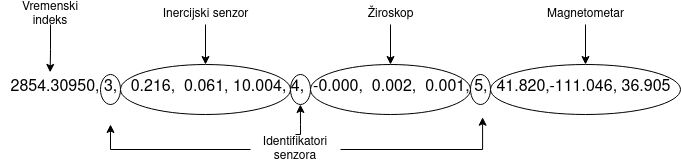
\includegraphics[width=\textwidth]{datagram.png}
    \caption{Primjerak primljenih podataka}
    \label{datagram}
\end{figure}

Kako bi se ti podaci primili i pohranili na adekvatan način potrebno je napraviti program klijent koji osluškuje na određenim portovima. Implementacija tog programa 
u ovome radu biti će napravljena koristeći skriptni jezik python. 


\section{Implementacija metode strojnoga učenja}

\section{Rezultati}

\chapter{Zaključak}
Zaključak.

\bibliography{literatura}
\bibliographystyle{fer}

\begin{sazetak}
Sažetak na hrvatskom jeziku.

\kljucnerijeci{Ključne riječi, odvojene zarezima.}
\end{sazetak}

% TODO: Navedite naslov na engleskom jeziku.
\engtitle{Title}
\begin{abstract}
Abstract.

\keywords{Keywords.}
\end{abstract}

\end{document}
